\documentclass{ximera}

%% You can put user macros here
%% However, you cannot make new environments

\listfiles

\graphicspath{{./}{firstExample/}{secondExample/}}

\usepackage{tikz}
\usepackage{tkz-euclide}
\usepackage{tikz-3dplot}
\usepackage{tikz-cd}
\usetikzlibrary{shapes.geometric}
\usetikzlibrary{arrows}
\usetikzlibrary{decorations.pathmorphing,patterns}
\usetkzobj{all}
\pgfplotsset{compat=1.13} % prevents compile error.

\renewcommand{\vec}[1]{\mathbf{#1}}
\newcommand{\RR}{\mathbb{R}}
\newcommand{\dfn}{\textit}
\newcommand{\dotp}{\cdot}
\newcommand{\id}{\text{id}}
\newcommand\norm[1]{\left\lVert#1\right\rVert}
 
\newtheorem{general}{Generalization}
\newtheorem{initprob}{Exploration Problem}

\tikzstyle geometryDiagrams=[ultra thick,color=blue!50!black]

\usepackage{mathtools}

\title{Separable Equations}


\begin{document}%\label{module1-A}

\begin{abstract}
We define what it means for a first order equation to be separable, and we work out solutions to a few examples of separable equations.
\end{abstract}

\maketitle

\section*{Separable Equations}


A first order differential equation  is  \dfn{separable} if it can be written as
\begin{equation} \label{eq:2.2.1}
h(y)y'=g(x),
\end{equation}
where the left side is a product of $y'$ and a function of $y$ and
the right side is a function of $x$. Rewriting a separable
differential equation in this form is called \dfn{separation of
variables}. 

%In {\color{red}Section~2.1} we used separation of variables
%to solve homogeneous linear equations. In this section we'll apply
%this method to nonlinear equations.

To see how to solve \eqref{eq:2.2.1}, let's first assume that $y$
is a solution.
Let  $G(x)$ and $H(y)$ be antiderivatives of $g(x)$
and $h(y)$; that is,
\begin{equation} \label{eq:2.2.2}
H'(y)=h(y)\quad\text{and}\quad G'(x)=g(x).
\end{equation}
Then, from the chain rule,
$$
\frac{d}{dx}H(y(x))=H'(y(x))y'(x)=h(y)y'(x).
$$
Therefore \eqref{eq:2.2.1} is equivalent to
$$
\frac{d}{dx}H(y(x))=\frac{d}{dx}G(x).
$$
Integrating both sides of this equation and combining the constants of
integration yields
\begin{equation} \label{eq:2.2.3}
H(y(x))=G(x)+c.
\end{equation}
Although we derived this equation on the assumption that $y$
is a solution of \eqref{eq:2.2.1}, we can now view it differently:
Any differentiable function $y$ that satisfies \eqref{eq:2.2.3}
for some constant $c$ is a solution of \eqref{eq:2.2.1}. To see this, we
differentiate both sides of \eqref{eq:2.2.3}, using the chain rule on the
left, to obtain
$$
H'(y(x))y'(x)=G'(x),
$$
which is equivalent to
$$
h(y(x))y'(x)=g(x)
$$
because of \eqref{eq:2.2.2}.

In conclusion, to solve \eqref{eq:2.2.1} it suffices to find
functions $G=G(x)$ and $H=H(y)$ that satisfy \eqref{eq:2.2.2}.
Then any differentiable function  $y=y(x)$  that satisfies
\eqref{eq:2.2.3} is a solution of \eqref{eq:2.2.1}.

\begin{example}\label{example:2.2.1}
Solve the equation
$$
y'=x(1+y^2).
$$
\begin{explanation}
Separating variables
yields
$$
\frac{y'}{1+y^2}=x.
$$
Integrating yields
$$
\tan^{-1}y=\frac{x^2}{2}+c
$$
Therefore
$$
y=\tan\left(\frac{x^2}{2}+c\right).
$$
\end{explanation}
\end{example}

\begin{example}\label{example:2.2.2} 
\begin{enumerate}
\item\label{item:2.2.2a}
Solve the equation
\begin{equation} \label{eq:2.2.4}
y'=-\frac{x}{y}.
\end{equation}

\item\label{item:2.2.2b}
Solve the initial value problem
\begin{equation} \label{eq:2.2.5}
y'=-\frac{x}{y}, \quad y(1)=1.
\end{equation}

\item \label{item:2.2.2c}
Solve the initial value problem
\begin{equation} \label{eq:2.2.6}
y'=-\frac{x}{y}, \quad y(1)=-2.
\end{equation}
\end{enumerate}

\begin{explanation}
\ref{item:2.2.2a} Separating variables
in \eqref{eq:2.2.4}  yields
$$
yy'=-x.
$$
Integrating yields
$$
\frac{y^2}{2}=-\frac{x^2}{2}+c,\quad\text{or, equivalently,}\quad
x^2+y^2=2c.
$$
The last equation shows that $c$ must be positive if $y$ is to be a
solution of \eqref{eq:2.2.4} on an open interval. Therefore we let
$2c=a^2$ (with $a > 0$) and rewrite the last equation as
\begin{equation} \label{eq:2.2.7}
x^2+y^2=a^2.
\end{equation}
 This equation has two differentiable solutions for $y$ in terms of
$x$:
\begin{equation} \label{eq:2.2.8}
y=\sqrt{a^2-x^2}, \quad -a < x < a,
\end{equation}
 and
\begin{equation} \label{eq:2.2.9}
y= - \sqrt{a^2-x^2}, \quad -a < x < a.
\end{equation}
The solution curves defined by \eqref{eq:2.2.8}  are semicircles
above the
$x$-axis and  those defined by \eqref{eq:2.2.9}  are semicircles below the
$x$-axis (Figure~\ref{figure:2.2.1}).

\ref{item:2.2.2b}  The solution of  \eqref{eq:2.2.5}
is positive when $x=1$; hence, it  is of the form \eqref{eq:2.2.8}.
 Substituting $x=1$ and $y=1$ into \eqref{eq:2.2.7} to satisfy the
initial condition yields $a^2=2$; hence, the solution of
\eqref{eq:2.2.5}
is
$$
y=\sqrt{2-x^2}, \quad - \sqrt{2}< x < \sqrt{2}.
$$

\ref{item:2.2.2c}  The solution of  \eqref{eq:2.2.6}
is negative when $x=1$ and   is therefore of the form \eqref{eq:2.2.9}.
 Substituting $x=1$ and $y=-2$ into \eqref{eq:2.2.7} to satisfy the
initial condition yields $a^2=\answer{5}$. Hence, the solution of \eqref{eq:2.2.6}
is
$$
y=-\sqrt{\answer{5}-x^2}, \quad -\sqrt{\answer{5}} < x < \sqrt{\answer{5}}.
$$


\begin{image}
  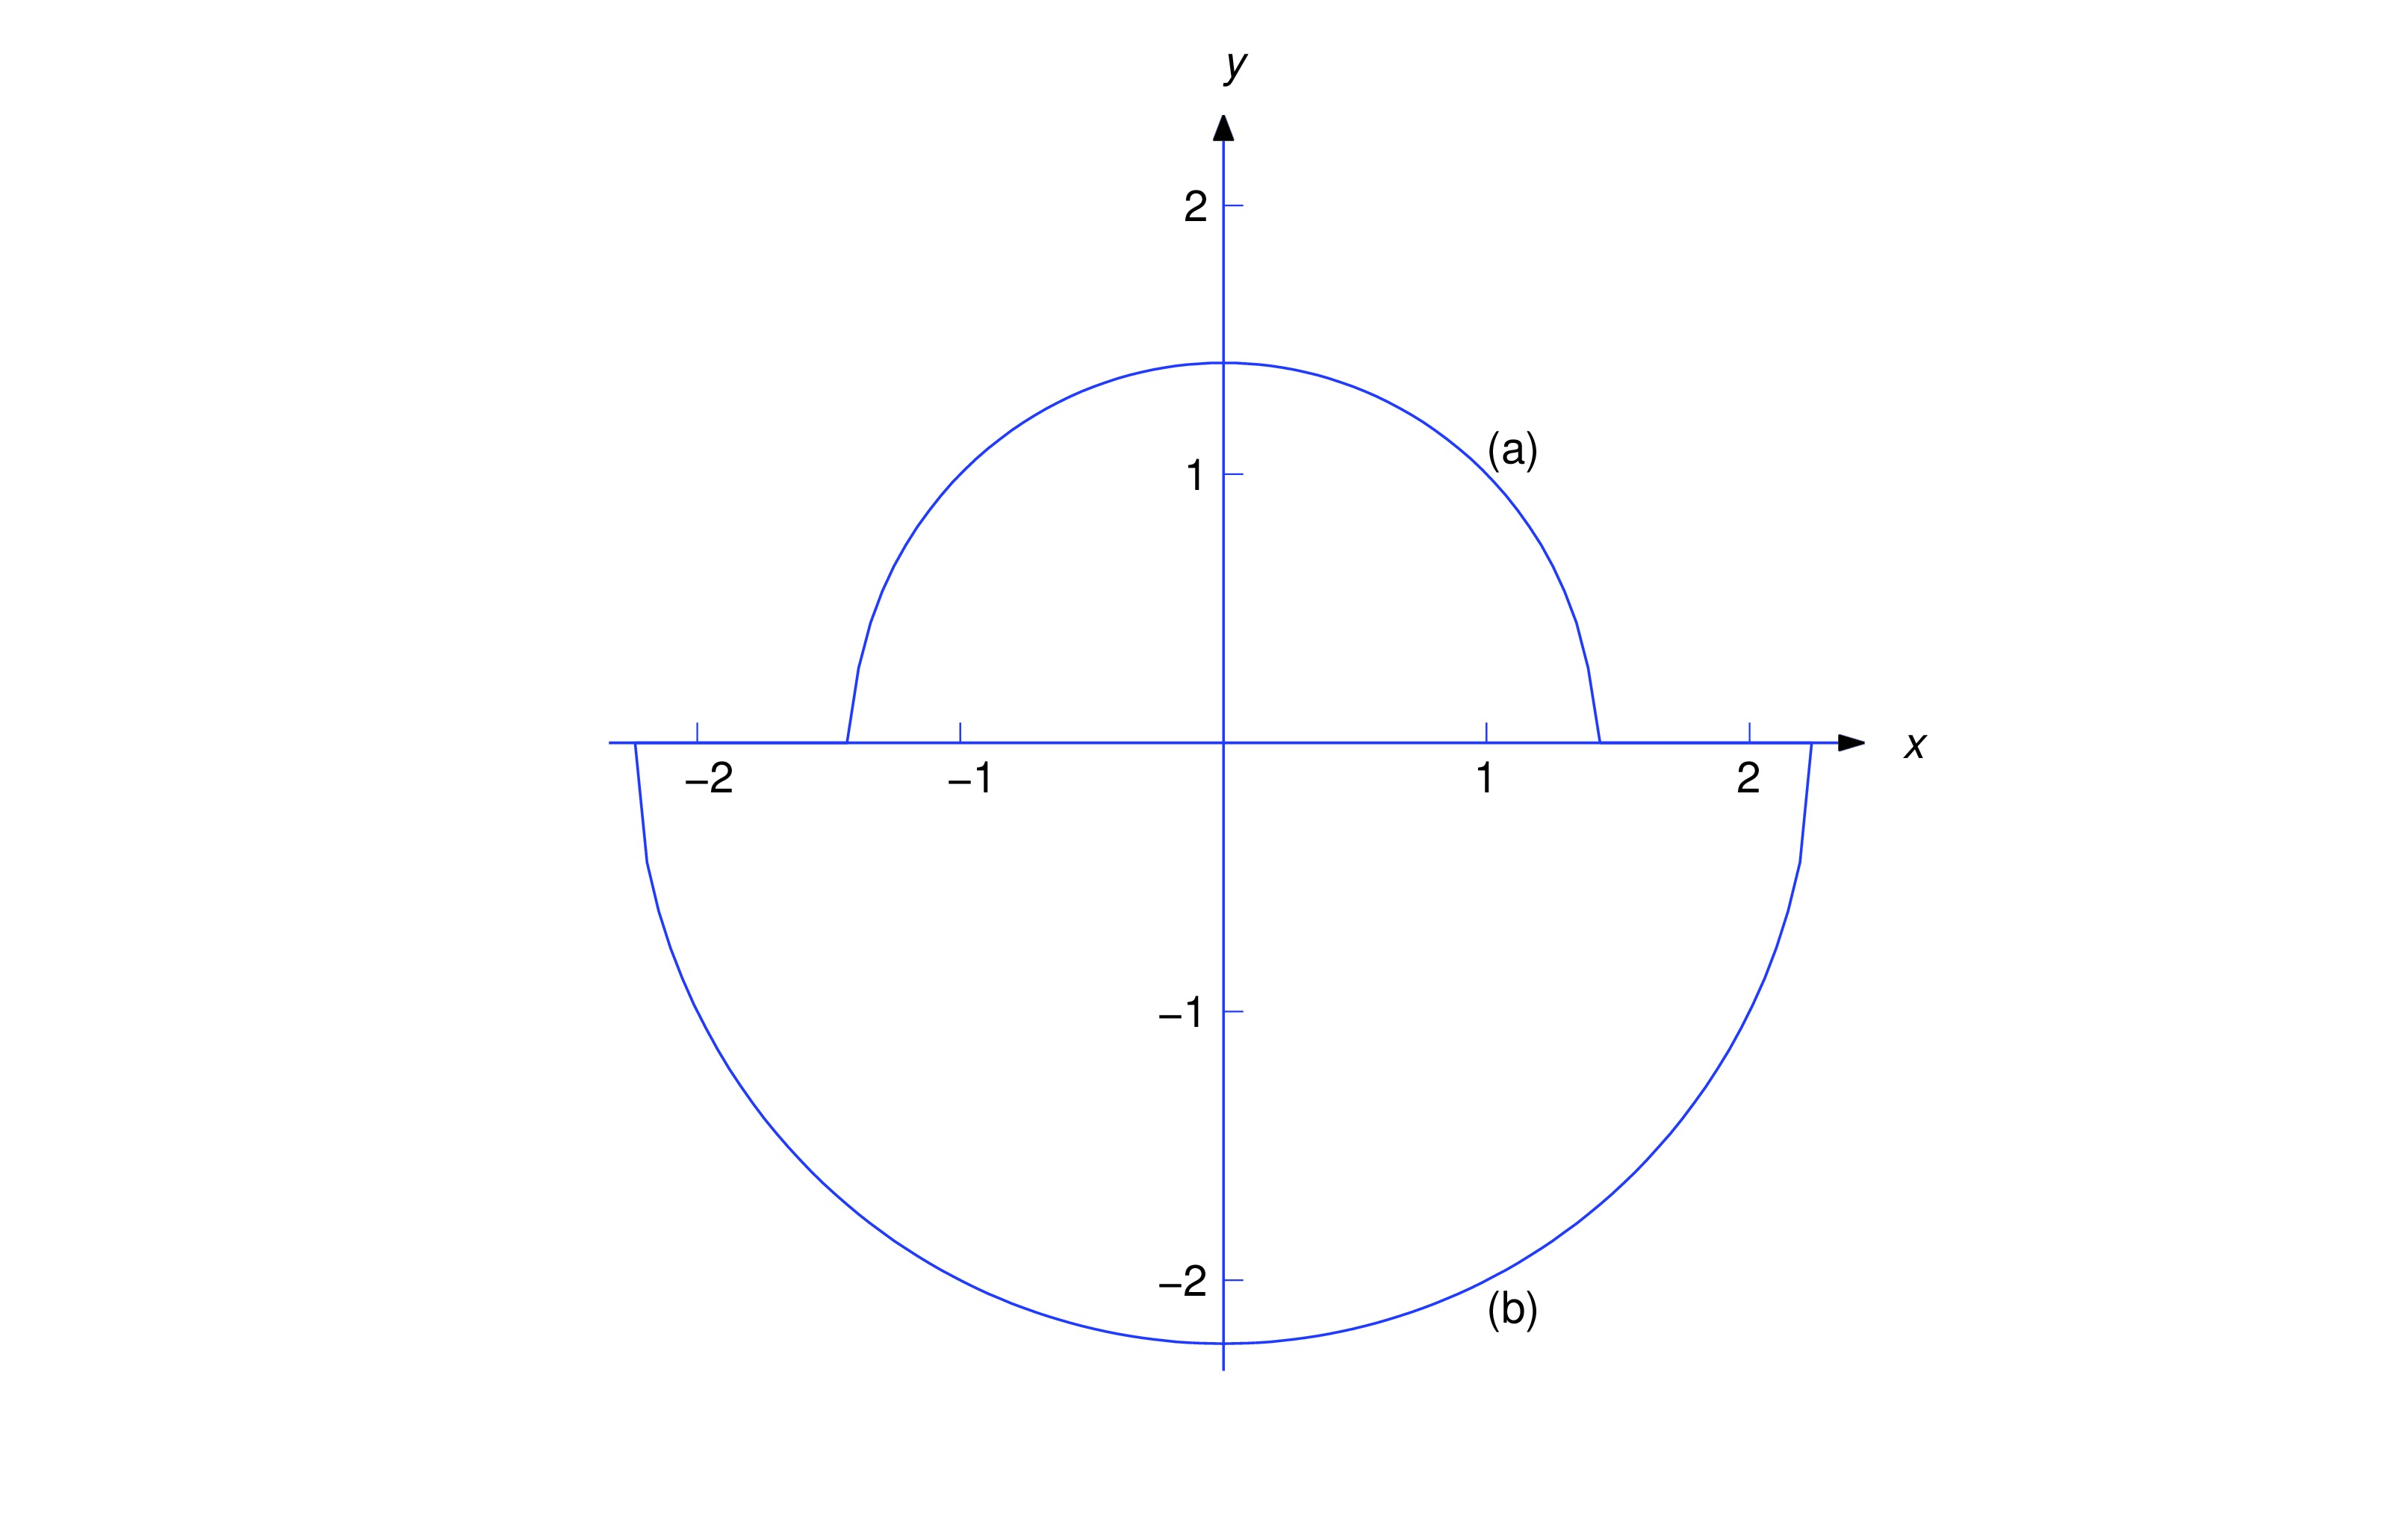
\includegraphics[height=1.5in]{fig020201.jpg}
\end{image}

\end{explanation}
\end{example}


\subsection*{Implicit Solutions of Separable Equations}


In Examples~\ref{example:2.2.1} and \ref{example:2.2.2} we were able to
solve the equation $H(y)=G(x)+c$ to obtain explicit formulas for
solutions of the given separable differential equations. As we'll
see in the next example, this isn't  always possible.
In this situation we must broaden our definition of a solution of a
separable equation. The next theorem provides the basis for this
modification.  We omit the proof, which requires a result from
advanced calculus called as the \dfn{implicit function
theorem}.

\begin{theorem}\label{thmtype:2.2.1}
Suppose $g=g(x)$ is continuous on $(a,b)$ and $h=h(y)$
are continuous on $(c,d)$. Let $G$ be an antiderivative of
$g$ on $(a,b)$ and let $H$ be an antiderivative of $h$ on $(c,d).$
Let $x_0$ be an arbitrary point in $(a,b),$ let $y_0$
be a point in $(c,d)$ such that $h(y_0)\neq 0,$ and define
\begin{equation} \label{eq:2.2.10}
c=H(y_0)-G(x_0).
\end{equation}
Then there's a function $y=y(x)$ defined on some open interval
$(a_1,b_1),$ where $a\leq a_1<x_0<b_1\leq b,$ such that  $y(x_0)=y_0$
and
\begin{equation} \label{eq:2.2.11}
H(y)=G(x)+c
\end{equation}
for $a_1<x<b_1$.
Therefore $y$ is a solution of the initial value problem
\begin{equation} \label{eq:2.2.12}
h(y)y'=g(x),\quad y(x_0)=x_0.
\end{equation}
\end{theorem}


It's convenient to say that \eqref{eq:2.2.11} with $c$ arbitrary is an
\dfn{implicit solution} of $h(y)y'=g(x)$. Curves defined by
\eqref{eq:2.2.11} are integral curves of $h(y)y'=g(x)$. If $c$ satisfies
\eqref{eq:2.2.10}, we'll say that \eqref{eq:2.2.11} is an \dfn{
implicit solution of the initial value problem} \eqref{eq:2.2.12}. However, keep
these  points in mind:
\begin{itemize}
\item  For some choices of $c$ there may not be any differentiable
functions $y$ that satisfy \eqref{eq:2.2.11}.
\item  The function $y$ in \eqref{eq:2.2.11} (not \eqref{eq:2.2.11} itself)
is a solution of $h(y)y'=g(x)$.
\end{itemize}

\begin{example}\label{example:2.2.3}
\begin{enumerate}
\item\label{item:2.2.3a}
Find implicit solutions of
\begin{equation} \label{eq:2.2.13}
y'=\frac{2x+1}{5y^4+1}.
\end{equation}
\item\label{item:2.2.3b}
Find an implicit solution of
\begin{equation} \label{eq:2.2.14}
y'=\frac{2x+1}{5y^4+1},\quad y(2)=1.
\end{equation}
\end{enumerate}

\begin{explanation}
\ref{item:2.2.3a}
 Separating variables yields
$$
(5y^4+1)y'=2x+1.
$$
Integrating yields the implicit solution
\begin{equation} \label{eq:2.2.15}
y^5+y=x^2+x+ c.
\end{equation}
of \eqref{eq:2.2.13}.

\ref{item:2.2.3b} Imposing the initial condition $y(2)=1$ in
\eqref{eq:2.2.15} yields $1+1=4+2+c$, so $c=-4$. Therefore
$$
y^5+y=x^2+x-4
$$
is an implicit solution of the initial value problem \eqref{eq:2.2.14}.
Although more than one differentiable function $y=y(x)$ satisfies
\ref{eq:2.2.13}) near $x=1$, it can be shown that there's only
one such function that satisfies the initial condition $y(1)=2$.

The figure below shows a direction field and some integral curves
for \eqref{eq:2.2.13}.

\begin{image}
    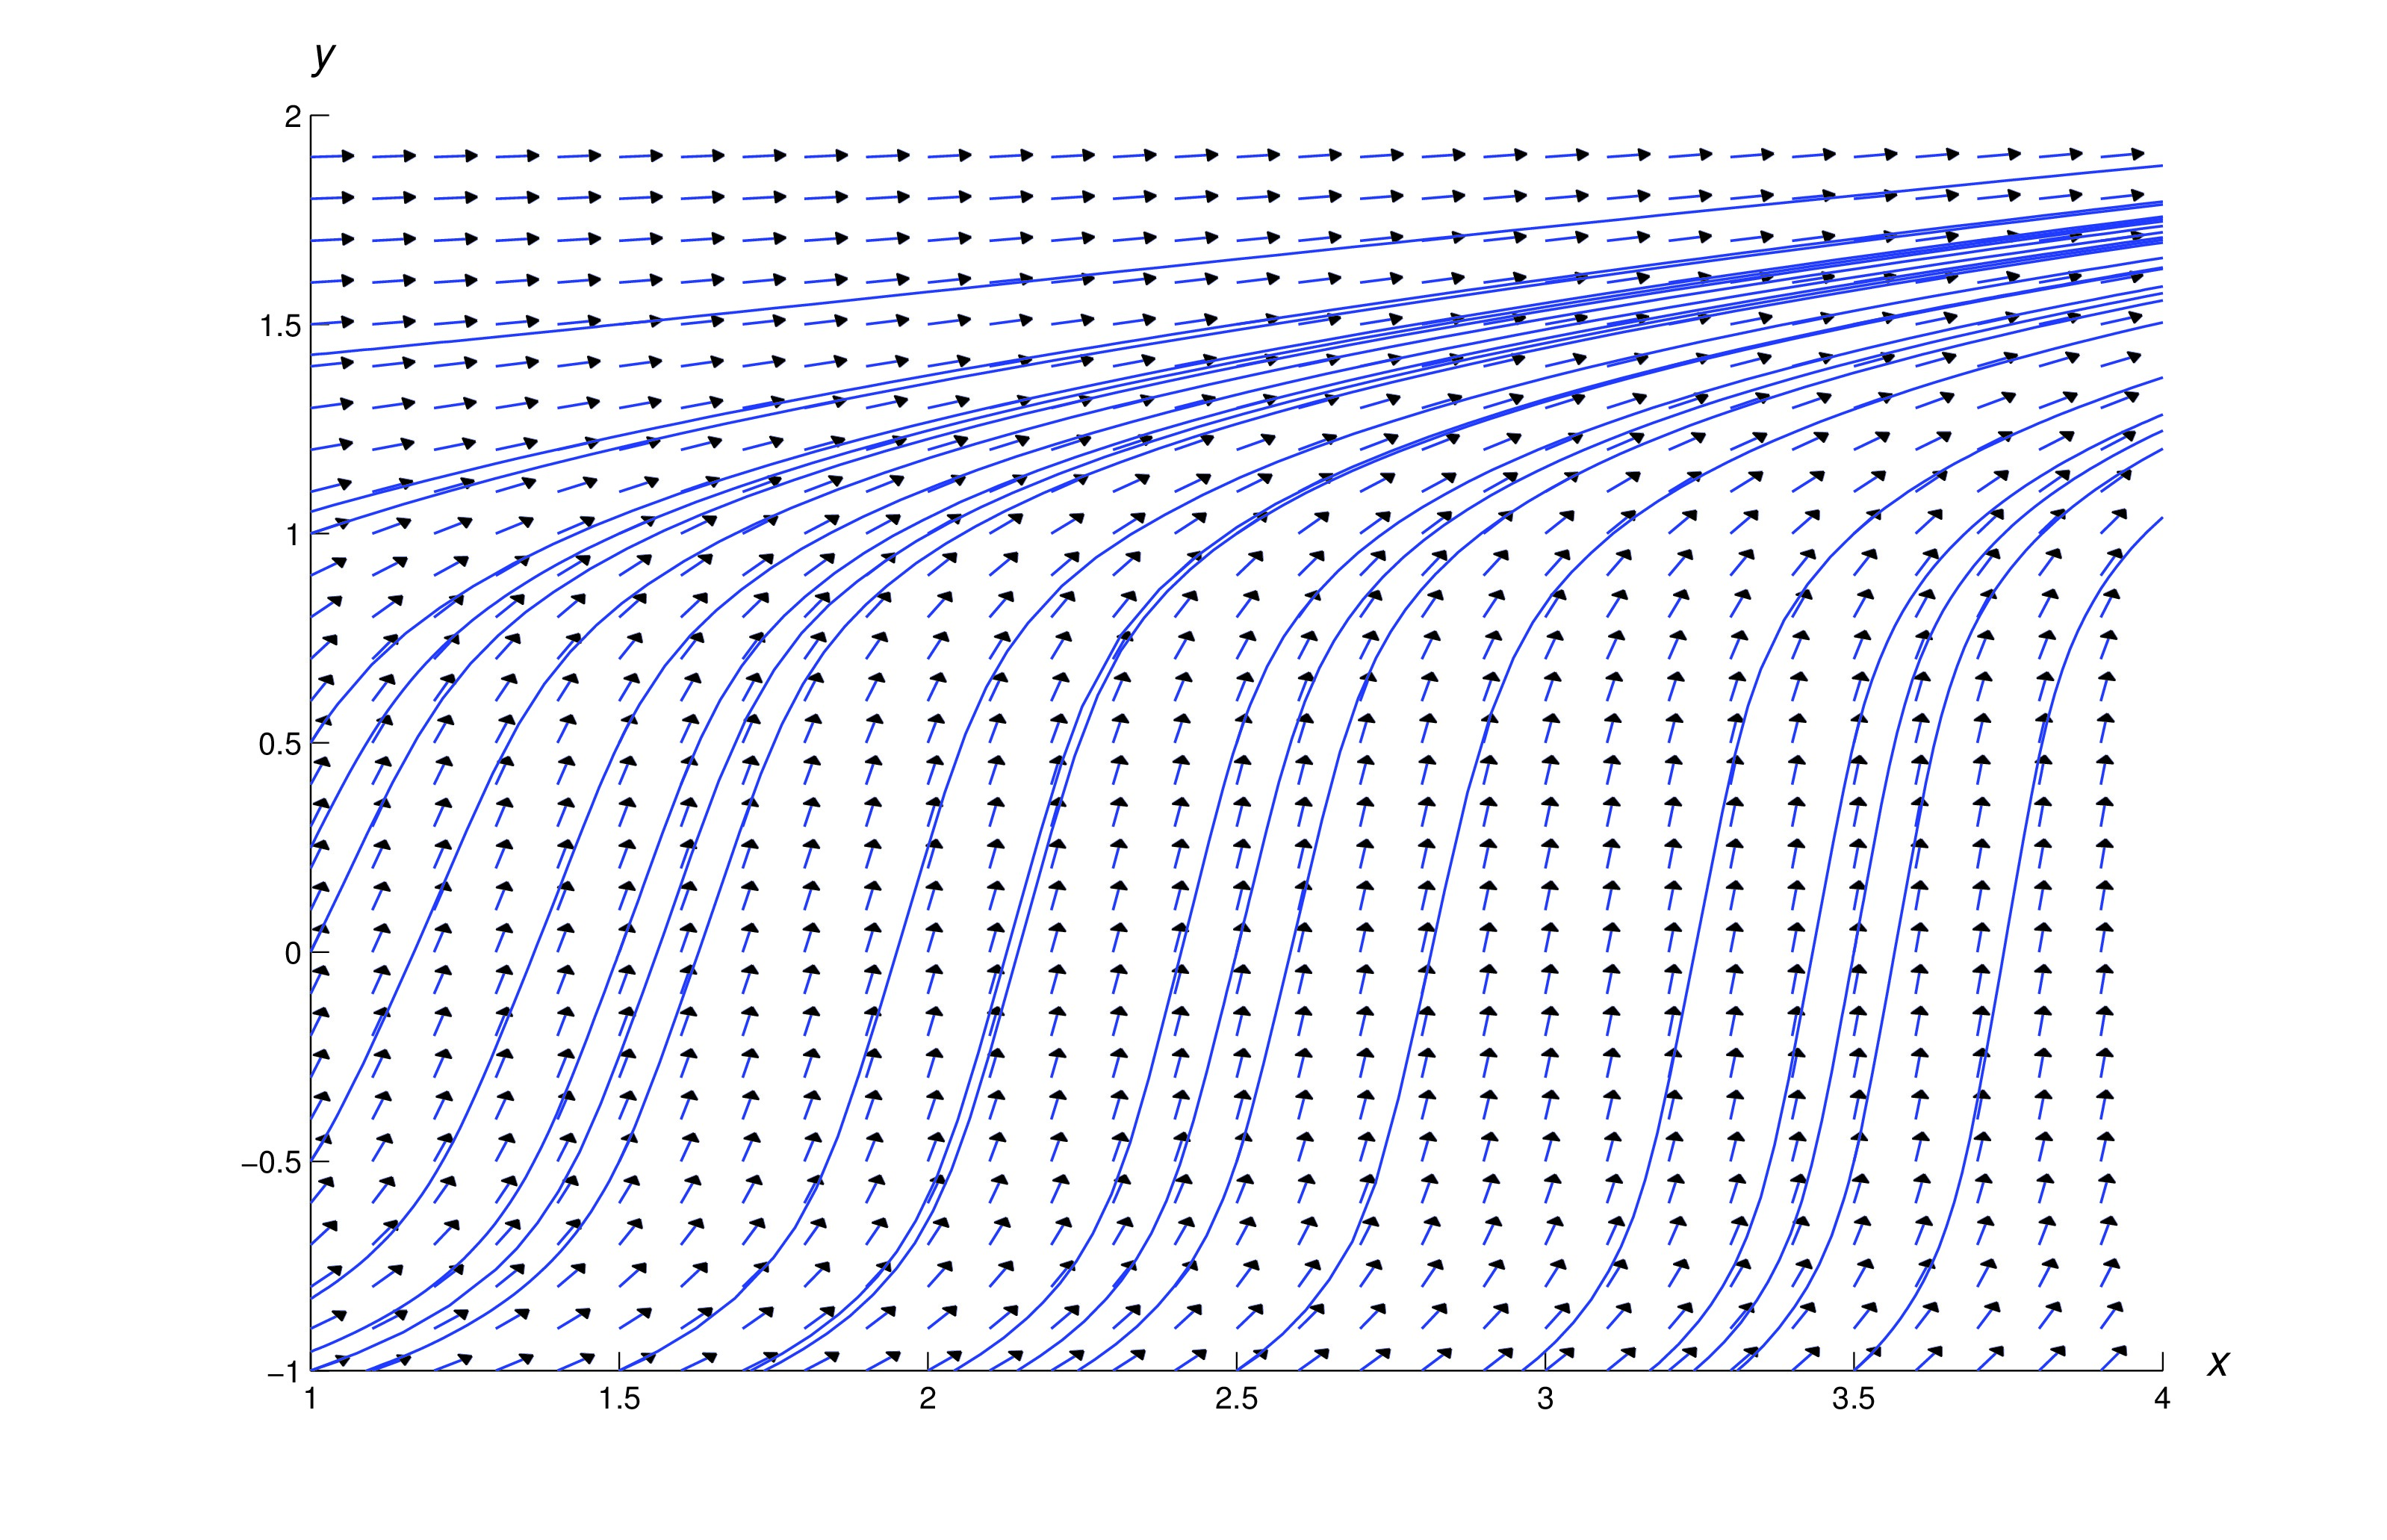
\includegraphics[height=1.5in]{fig020202.jpg}
\end{image}

\end{explanation}
\end{example}

\subsection*{Constant Solutions of Separable Equations}

An equation of the form
$$
y'=g(x)p(y)
$$
 is separable, since it can be rewritten as
$$
\frac{1}{p(y)}y'=g(x).
$$
 However, the division by  $p(y)$
is not legitimate  if $p(y)=0$ for some values of $y$.  The
next two examples show how to deal with this problem.

\begin{example}\label{example:2.2.4}
Find all solutions of
\begin{equation} \label{eq:2.2.16}
y'=2xy^2.
\end{equation}

\begin{explanation} 
Here we must divide by $p(y)=y^2$ to separate variables.
This isn't  legitimate if $y$ is a solution of \eqref{eq:2.2.16} that
equals zero for some value of $x$. One such solution can be found by
inspection:  $y \equiv 0$. Now suppose   $y$ is a solution
of \eqref{eq:2.2.16} that isn't  identically zero. Since $y$ is continuous there must be an interval on which $y$ is never zero. Since division
by $y^2$ is legitimate for $x$ in this interval, we can separate
variables in \eqref{eq:2.2.16} to obtain
$$
\frac{y'}{y^2}=2x.
$$
 Integrating this yields
$$
-\frac{1}{y}=x^2+c,
$$
which is equivalent to
\begin{equation} \label{eq:2.2.17}
y=-\frac{1}{x^2+c}.
\end{equation}

We've now shown that if $y$ is a solution of \eqref{eq:2.2.16} that is
not identically zero, then $y$ must be of the form \eqref{eq:2.2.17}. By
substituting \eqref{eq:2.2.17} into \eqref{eq:2.2.16}, you can verify that
\eqref{eq:2.2.17} is  a solution of \eqref{eq:2.2.16}. Thus,
 solutions of \eqref{eq:2.2.16} are $y\equiv 0$ and the functions
of the form \eqref{eq:2.2.17}. Note that the solution $y\equiv 0$ isn't  of
the form \eqref{eq:2.2.17} for any value of $c$.

The figure below shows a direction field and some integral
curves for \eqref{eq:2.2.16}


\begin{image}
  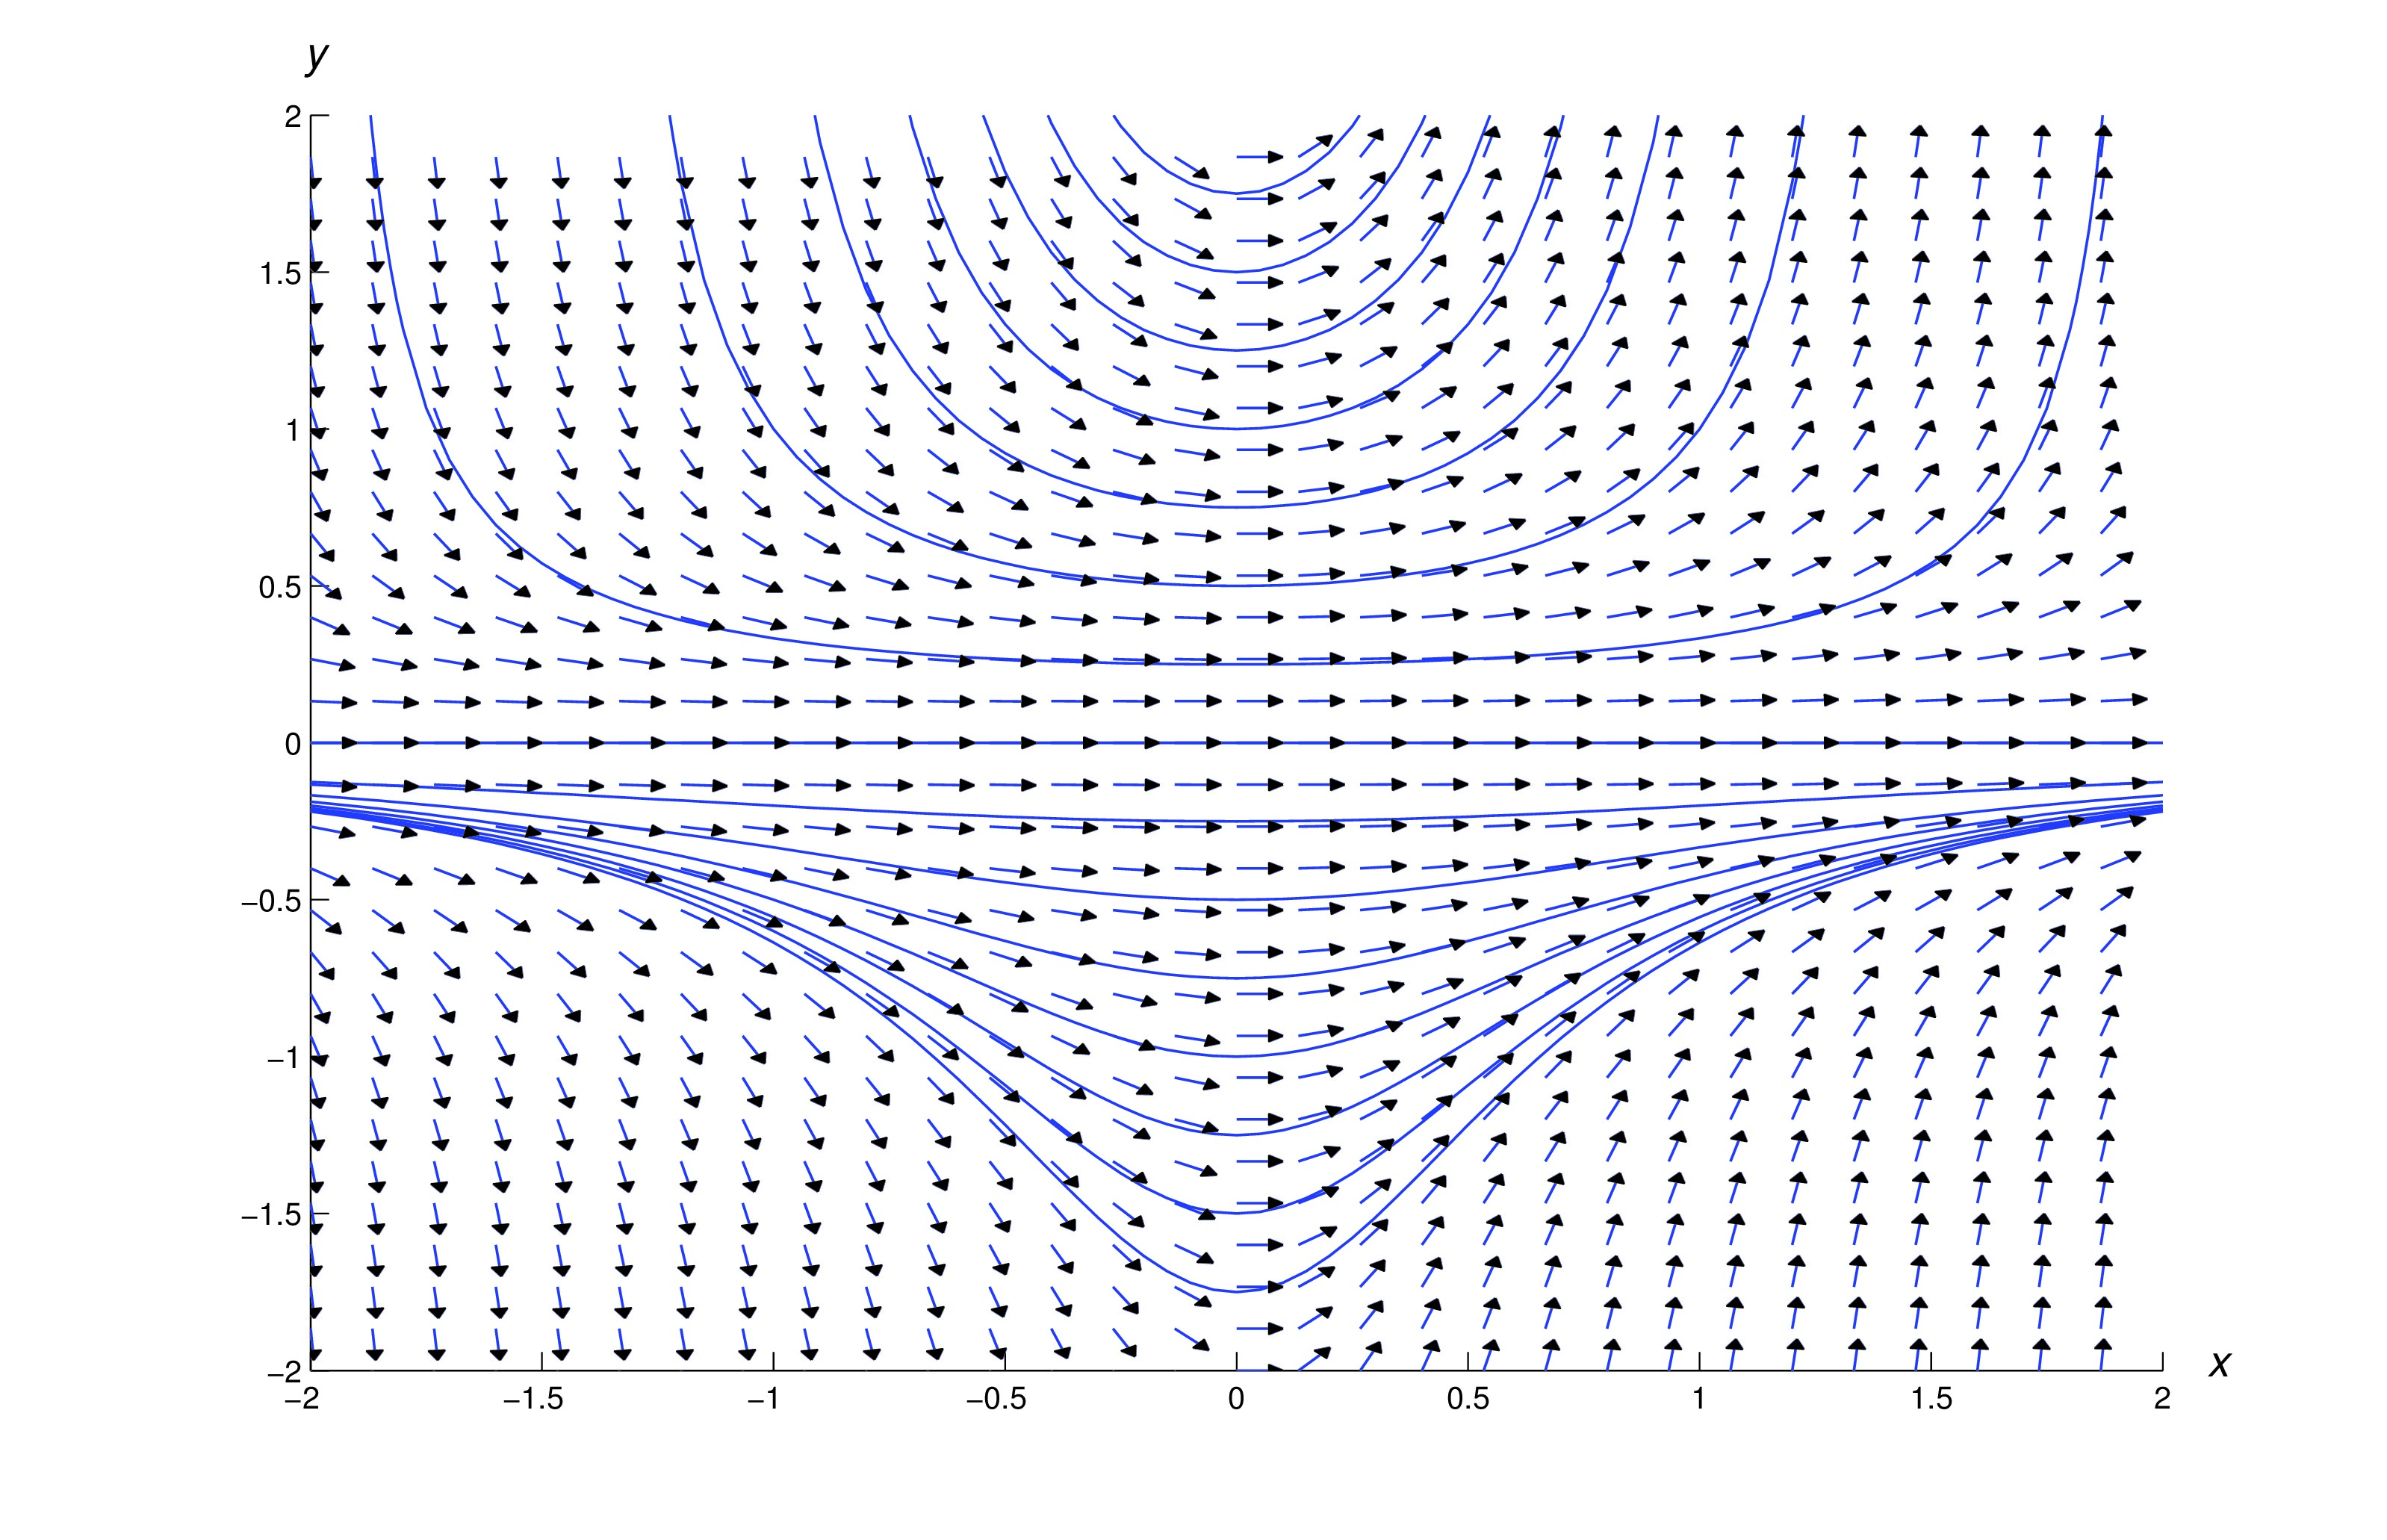
\includegraphics[height=1.5in]{fig020203.jpg}
\end{image}
\end{explanation}
\end{example}

\begin{example}\label{example:2.2.5}
Find all solutions of
\begin{equation} \label{eq:2.2.18}
y'=\frac{1}{2}x(1-y^2).
\end{equation}

\begin{explanation}

Here we must divide by $p(y)=1-y^2$ to separate variables.
This isn't  legitimate if $y$ is a solution of \eqref{eq:2.2.18} that
equals $\pm 1$ for some value of $x$. Two such solutions can be found
by inspection: $y \equiv 1$ and $y\equiv -1$. Now suppose
$y$ is a solution of \eqref{eq:2.2.18} such that $1-y^2$ isn't
identically zero. Since $1-y^2$ is continuous there must be an
interval on which $1-y^2$ is never zero. Since division by $1-y^2$ is
legitimate for $x$ in this interval, we can separate variables in
\eqref{eq:2.2.18} to obtain
$$
\frac{2y'}{y^2-1}=-x.
$$
 A partial fraction expansion on the left yields
$$
\left[\frac{1}{y-1}-\frac{1}{y+1}\right]y'=-x,
$$
and integrating  yields
$$
\ln\left|\frac{y-1}{y+1}\right|=-\frac{x^2}{2}+k;
$$
 hence,
$$
\left|\frac{y-1}{y+1}\right|=e^ke^{-x^2/2}.
$$
 Since $y(x)\neq \pm 1$ for $x$ on the interval under discussion, the
quantity
$(y-1)/(y+1)$  can't  change sign in this interval. Therefore
we can rewrite the last equation as
$$
\frac{y-1}{y+1}=ce^{-x^2/2},
$$
  where $c=\pm e^k$, depending upon the sign of $(y-1)/(y+1)$ on the
interval.
 Solving for  $y$ yields
\begin{equation} \label{eq:2.2.19}
y=\frac{1+ce^{-x^2/2}}{1-ce^{-x^2/2}}.
\end{equation}

We've now shown that if $y$ is a solution of \eqref{eq:2.2.18} that  is
not identically equal to $\pm 1$, then $y$ must be as in
\eqref{eq:2.2.19}. By substituting \eqref{eq:2.2.19} into \eqref{eq:2.2.18} you
 can verify that \eqref{eq:2.2.19} is  a solution of
\eqref{eq:2.2.18}. Thus,  the solutions of \eqref{eq:2.2.18}
are $y\equiv 1$, $y\equiv -1$ and the functions of the form
\eqref{eq:2.2.19}. Note that the constant solution $y \equiv 1$ can be
obtained from this formula by taking $c=0$;     however, the other
constant solution, $y \equiv -1$, can't be obtained in this way.

The figure below shows a direction field and some integrals for
\eqref{eq:2.2.18}.


\begin{image}
  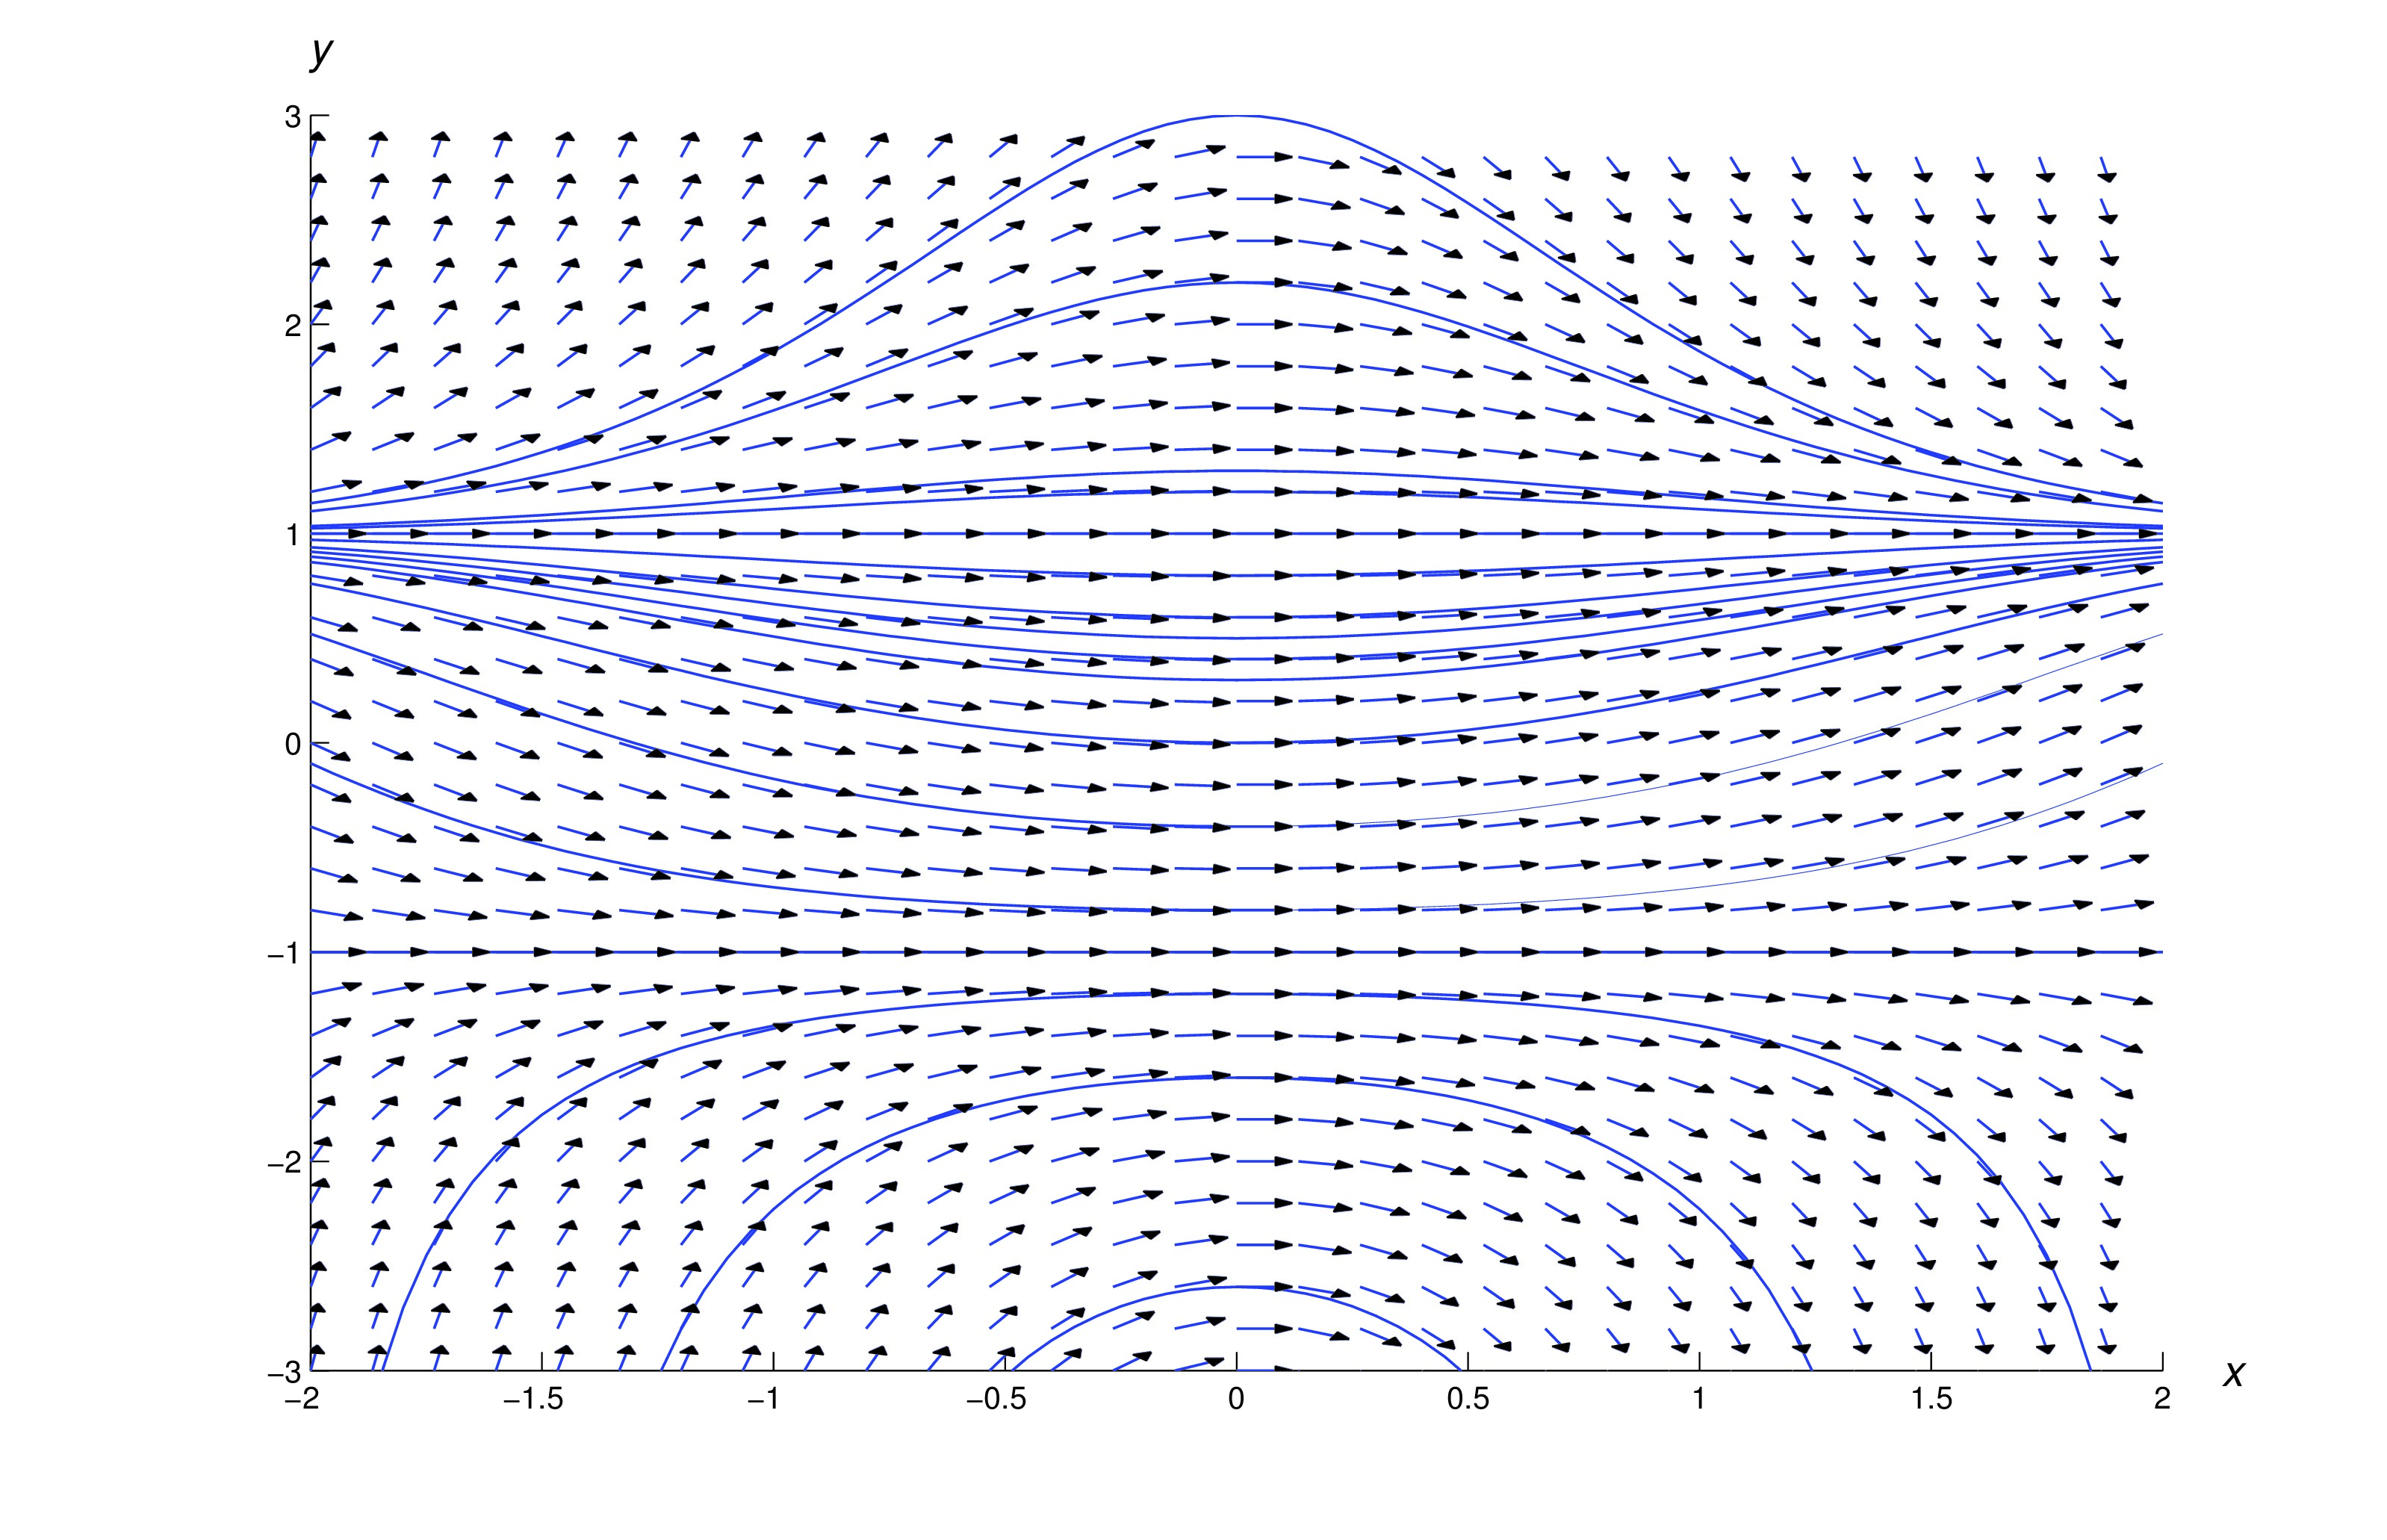
\includegraphics[height=1.5in]{fig020204.jpg}
\end{image}
\end{explanation}
\end{example}

% \subsection*{Differences Between Linear and Nonlinear Equations}

% Theorem~\ref{thmtype:2.1.2} states that if $p$ and $f$ are continuous on
% $(a,b)$ then every solution of
% $$
% y'+p(x)y=f(x)
% $$
%  on  $(a,b)$  can be obtained by choosing a value for the constant
% $c$  in the general solution, and   if
% $x_0$ is any point in  $(a,b)$ and $y_0$ is arbitrary, then the
% initial value problem
% $$
% y'+p(x)y=f(x),\quad y(x_0)=y_0
% $$
%  has a solution on  $(a,b)$.

% The not true for nonlinear equations. First, we
% saw in Examples~\ref{example:2.2.4} and \ref{example:2.2.5} that a
% nonlinear
% equation may have solutions that can't be obtained by choosing a
% specific value of a constant appearing in a one-parameter family of
% solutions. Second, it is in general impossible to determine the
% interval of validity of a solution to an initial value problem for a
% nonlinear equation by simply examining the equation, since the
% interval of validity may depend on the initial condition. For
% instance, in Example~\ref{example:2.2.2} we saw that the solution of
% $$
% \frac{dy}{dx}=-\frac{x}{y},\quad y(x_0)=y_0
% $$
% is valid on $(-a,a)$, where $a=\sqrt{x_0^2+y_0^2}$.

% \begin{example}\label{example:2.2.6}
% Solve the initial value problem
% $$
% y'=2xy^2, \quad y(0)=y_0
% $$
%  and determine the  interval of validity of  the solution.

% \begin{explanation} First suppose   $y_0\neq 0$. From
% Example~\ref{example:2.2.4}, we know that $y$ must be of the form
% \begin{equation} \label{eq:2.2.20}
% y=-\frac{1}{x^2+c}.
% \end{equation}
%  Imposing the initial condition shows  that $c=-1/y_0$.
% Substituting this into \eqref{eq:2.2.20} and rearranging terms yields
% the solution
% $$
% y= \frac{y_0}{1-y_0x^2}.
% $$
% This is also the solution if $y_0=0$. If $y_0<0$,
% the denominator isn't  zero for any value of $x$, so the
% the solution is valid on $(-\infty,\infty)$. If $y_0>0$, the solution
%  is  valid only on $(-1/\sqrt{y_0},1/\sqrt{y_0})$.
%  \end{explanation}
% \end{example}

\section*{Text Source}
Trench, William F., "Elementary Differential Equations" (2013). Faculty Authored and Edited Books \& CDs. 8. (CC-BY-NC-SA)

\href{https://digitalcommons.trinity.edu/mono/8/}{https://digitalcommons.trinity.edu/mono/8/}

\end{document}
